\documentclass[11pt]{article}

\usepackage[margin=1in]{geometry}
\usepackage{amsmath,amssymb,amsthm}
\usepackage{graphicx}
\usepackage{booktabs}
\usepackage{microtype}
\usepackage{natbib}
\usepackage[colorlinks=true,allcolors=RoyalBlue]{hyperref}
\usepackage[usenames,dvipsnames]{xcolor}
\usepackage{caption}
\usepackage{subcaption}
\usepackage{xspace}

% Headline numbers, generated from the campaign JSON by
% experiments.measurement_cot.numbers. Never edited by hand.
% Generated by experiments.measurement_cot.numbers -- do not edit by hand.
% Every figure quoted in the prose is defined here from the campaign JSON.
\providecommand{\BottleneckArgmax}{}\renewcommand{\BottleneckArgmax}{0.713\xspace}
\providecommand{\BottleneckContinuous}{}\renewcommand{\BottleneckContinuous}{0.981\xspace}
\providecommand{\BottleneckMax}{}\renewcommand{\BottleneckMax}{0.986\xspace}
\providecommand{\BottleneckMeanSpread}{}\renewcommand{\BottleneckMeanSpread}{0.521\xspace}
\providecommand{\BottleneckMin}{}\renewcommand{\BottleneckMin}{0.456\xspace}
\providecommand{\BottleneckNoFeedback}{}\renewcommand{\BottleneckNoFeedback}{0.461\xspace}
\providecommand{\BottleneckPause}{}\renewcommand{\BottleneckPause}{0.460\xspace}
\providecommand{\BottleneckSampleOne}{}\renewcommand{\BottleneckSampleOne}{0.479\xspace}
\providecommand{\BottleneckSampleSixteen}{}\renewcommand{\BottleneckSampleSixteen}{0.730\xspace}
\providecommand{\BottleneckSpread}{}\renewcommand{\BottleneckSpread}{0.530\xspace}
\providecommand{\CapacityFloorAccuracy}{}\renewcommand{\CapacityFloorAccuracy}{0.482\xspace}
\providecommand{\CapacityFloorDim}{}\renewcommand{\CapacityFloorDim}{16\xspace}
\providecommand{\CapacityPeakDim}{}\renewcommand{\CapacityPeakDim}{64\xspace}
\providecommand{\CapacityPeakGap}{}\renewcommand{\CapacityPeakGap}{0.068\xspace}
\providecommand{\CapacityWideGap}{}\renewcommand{\CapacityWideGap}{0.003\xspace}
\providecommand{\DepthArgmaxDeep}{}\renewcommand{\DepthArgmaxDeep}{0.589\xspace}
\providecommand{\DepthArgmaxShallow}{}\renewcommand{\DepthArgmaxShallow}{0.827\xspace}
\providecommand{\DepthContinuousMax}{}\renewcommand{\DepthContinuousMax}{0.981\xspace}
\providecommand{\DepthContinuousMin}{}\renewcommand{\DepthContinuousMin}{0.947\xspace}
\providecommand{\DepthDeep}{}\renewcommand{\DepthDeep}{5\xspace}
\providecommand{\DepthFrontierDeep}{}\renewcommand{\DepthFrontierDeep}{21\xspace}
\providecommand{\DepthFrontierShallow}{}\renewcommand{\DepthFrontierShallow}{4\xspace}
\providecommand{\DepthGapDeep}{}\renewcommand{\DepthGapDeep}{0.386\xspace}
\providecommand{\DepthGapShallow}{}\renewcommand{\DepthGapShallow}{0.143\xspace}
\providecommand{\DepthSampleEightDeep}{}\renewcommand{\DepthSampleEightDeep}{0.539\xspace}
\providecommand{\DepthSampleEightShallow}{}\renewcommand{\DepthSampleEightShallow}{0.856\xspace}
\providecommand{\DepthShallow}{}\renewcommand{\DepthShallow}{2\xspace}
\providecommand{\FrontierChance}{}\renewcommand{\FrontierChance}{0.070\xspace}
\providecommand{\FrontierMassContinuous}{}\renewcommand{\FrontierMassContinuous}{0.45\xspace}
\providecommand{\FrontierMassDiscrete}{}\renewcommand{\FrontierMassDiscrete}{0.39\xspace}
\providecommand{\JensenGapRatio}{}\renewcommand{\JensenGapRatio}{0.98\xspace}
\providecommand{\JensenHighEntropy}{}\renewcommand{\JensenHighEntropy}{3.56\xspace}
\providecommand{\JensenLowEntropy}{}\renewcommand{\JensenLowEntropy}{3.13\xspace}
\providecommand{\JensenQuadraticError}{}\renewcommand{\JensenQuadraticError}{1.8\xspace}
\providecommand{\MCFirstDistance}{}\renewcommand{\MCFirstDistance}{0.96\xspace}
\providecommand{\MCFirstSamples}{}\renewcommand{\MCFirstSamples}{1\xspace}
\providecommand{\MCLastDistance}{}\renewcommand{\MCLastDistance}{0.084\xspace}
\providecommand{\MCLastSamples}{}\renewcommand{\MCLastSamples}{128\xspace}
\providecommand{\MCObservedRatio}{}\renewcommand{\MCObservedRatio}{11.5\xspace}
\providecommand{\MCPredictedRatio}{}\renewcommand{\MCPredictedRatio}{11.3\xspace}
\providecommand{\NumSeeds}{}\renewcommand{\NumSeeds}{3\xspace}
\providecommand{\NumTestQueries}{}\renewcommand{\NumTestQueries}{3258\xspace}
\providecommand{\NumTrainQueries}{}\renewcommand{\NumTrainQueries}{7602\xspace}
\providecommand{\OpenArgmax}{}\renewcommand{\OpenArgmax}{0.969\xspace}
\providecommand{\OpenContinuous}{}\renewcommand{\OpenContinuous}{0.970\xspace}
\providecommand{\OpenMax}{}\renewcommand{\OpenMax}{0.975\xspace}
\providecommand{\OpenMeanSpread}{}\renewcommand{\OpenMeanSpread}{0.005\xspace}
\providecommand{\OpenMin}{}\renewcommand{\OpenMin}{0.961\xspace}
\providecommand{\OpenNoFeedback}{}\renewcommand{\OpenNoFeedback}{0.966\xspace}
\providecommand{\OpenPause}{}\renewcommand{\OpenPause}{0.967\xspace}
\providecommand{\OpenSampleOne}{}\renewcommand{\OpenSampleOne}{0.970\xspace}
\providecommand{\OpenSampleSixteen}{}\renewcommand{\OpenSampleSixteen}{0.971\xspace}
\providecommand{\OpenSpread}{}\renewcommand{\OpenSpread}{0.014\xspace}
\providecommand{\QuarterArgmax}{}\renewcommand{\QuarterArgmax}{0.957\xspace}
\providecommand{\QuarterContinuous}{}\renewcommand{\QuarterContinuous}{0.988\xspace}
\providecommand{\QuarterMax}{}\renewcommand{\QuarterMax}{0.992\xspace}
\providecommand{\QuarterMeanSpread}{}\renewcommand{\QuarterMeanSpread}{0.041\xspace}
\providecommand{\QuarterMin}{}\renewcommand{\QuarterMin}{0.944\xspace}
\providecommand{\QuarterNoFeedback}{}\renewcommand{\QuarterNoFeedback}{0.983\xspace}
\providecommand{\QuarterPause}{}\renewcommand{\QuarterPause}{0.983\xspace}
\providecommand{\QuarterSampleOne}{}\renewcommand{\QuarterSampleOne}{0.947\xspace}
\providecommand{\QuarterSampleSixteen}{}\renewcommand{\QuarterSampleSixteen}{0.974\xspace}
\providecommand{\QuarterSpread}{}\renewcommand{\QuarterSpread}{0.048\xspace}
\providecommand{\SchedAlternating}{}\renewcommand{\SchedAlternating}{0.755\xspace}
\providecommand{\SchedAlways}{}\renewcommand{\SchedAlways}{0.713\xspace}
\providecommand{\SchedEarly}{}\renewcommand{\SchedEarly}{0.792\xspace}
\providecommand{\SchedLate}{}\renewcommand{\SchedLate}{0.669\xspace}
\providecommand{\SchedNeverCollapse}{}\renewcommand{\SchedNeverCollapse}{0.981\xspace}
\providecommand{\TerminalShortcut}{}\renewcommand{\TerminalShortcut}{0.45\xspace}
\providecommand{\ZenoEntropyEnd}{}\renewcommand{\ZenoEntropyEnd}{1.65\xspace}
\providecommand{\ZenoEntropyStart}{}\renewcommand{\ZenoEntropyStart}{3.34\xspace}
\providecommand{\ZenoFrontierEnd}{}\renewcommand{\ZenoFrontierEnd}{0.819\xspace}
\providecommand{\ZenoFrontierStart}{}\renewcommand{\ZenoFrontierStart}{0.510\xspace}
\providecommand{\ZenoRepeats}{}\renewcommand{\ZenoRepeats}{12\xspace}


\captionsetup{font=small,labelfont=bf}
\bibliographystyle{plainnat}

\newtheorem{proposition}{Proposition}
\newtheorem{corollary}{Corollary}
\theoremstyle{definition}
\newtheorem{remark}{Remark}

\newcommand{\CBS}{\gamma}
\newcommand{\Ev}{\Phi}
\newcommand{\Exp}{\mathbb{E}}
\newcommand{\Cov}{\operatorname{Cov}}
\newcommand{\tr}{\operatorname{tr}}

\title{\textbf{Chain of Thought as Repeated Measurement}\\[2mm]
\large Discrete and continuous reasoning are one Tensor Brain operator\\
at two settings of a collapse dial}

\author{Tensor Brain research note}
\date{}

\begin{document}
\maketitle

\begin{abstract}
Chain-of-thought (CoT) reasoning emits a discrete token at every step; continuous
latent reasoning, of which COCONUT \citep{hao2024coconut} is the canonical
instance, feeds a hidden state back instead and is reported to keep several
candidate continuations alive at once. We observe that the Tensor Brain (TB)
already contains both operations, and contains them as \emph{one} operation. The
TB measurement $q \leftarrow \alpha q + \beta a_k$ writes a single sampled index
embedding back into the workspace; TB attention
$q \leftarrow q + \beta \sum_k p_k a_k$ writes the expectation, and the QTB draft
\citep{tresp2025bayes} already calls the latter a degenerate measurement whose
outcome is not revealed. Discrete and continuous chains of thought are therefore
the sharp and degenerate limits of a single update, and everything between them
is reachable by turning one knob.

Making that identification lets us ask a question the LLM literature cannot easily
pose, because in a transformer the token bottleneck is not adjustable: \emph{when
does measurement sharpness matter at all?} The TB retain gate $\alpha$ answers it.
At $\alpha = 1$ the entire latent state survives the step and, we find, every
collapse mode from a single sampled symbol to the exact expectation performs
identically (spanning just \OpenMeanSpread on our task). Sharpness only becomes a
variable once $\alpha$ shrinks and the step boundary turns into a real channel. At
$\alpha = 0$ the same conditions spread over \BottleneckMin--\BottleneckMax,
ordered exactly by how much the collapse operator can push through that channel.
\textbf{Sharpness is not a property of a reasoning style; it is a property of a
channel, and it only matters when there is one.} Narrowing the surviving state at
$\alpha = 1$ partially reopens the gap, confirming that what matters is boundary
capacity --- but only partially, which is itself informative: a narrow continuous
state and a sharp symbol are not interchangeable, because the first can still carry a
superposition and the second cannot.

We then quantify the gap between the two limits. In unitary quantum computation
measurements may always be deferred to the end of a circuit; in the TB the
evolution operator is nonlinear, so measurement and evolution do not commute, and
the discrepancy is exactly a Jensen gap. We prove it vanishes if and only if the
evolution is affine, give its second-order form
$\tfrac{1}{2}\beta^{2}\tr(\nabla^{2}\Ev\,\Cov_p[a])$, and confirm the predicted
$\beta^{2}$ scaling to within \JensenQuadraticError\% numerically. The companion
prediction --- that the gap shrinks as the chain grows confident --- holds when the
candidate spread is swept directly, but is \emph{flat} across the trained chain's own
steps, because on a search task the chain never becomes confident enough for the term
to move. Collapse is never cheap here, which is why no annealed schedule we tried
beats staying continuous. The same expansion separates two things the literature often
conflates: averaging $M$ measurements \emph{inside} a step converges to continuous
thought at rate $M^{-1/2}$, whereas self-consistency averages \emph{across} whole
chains and does not converge to it at all --- the two differ by the accumulated
Jensen gap. Finally, because the TB index layer exists at every step by
construction, the superposition that latent reasoning is supposed to maintain can
simply be read off rather than probed for, and repeated measurement of a single
concept window --- deliberation that costs no evolution steps --- is shown to
sharpen the index distribution \emph{towards} the true search frontier.

All experiments are from-scratch models on a synthetic multi-hop reachability task
and run in under an hour on a laptop CPU.
\end{abstract}

\section{Introduction}

A chain of thought is usually described as a sequence of intermediate results that
a model writes down before answering \citep{wei2022cot}. Written down is the
operative phrase: each step is forced through the vocabulary, so whatever the model
was entertaining collapses to one token before the next step begins. COCONUT
\citep{hao2024coconut} removes that constraint by feeding the last hidden state
back as the next input embedding, and reports that the resulting continuous thought
behaves like a breadth-first search, keeping several candidate next steps alive
where discrete decoding would have committed. The effect is large and it is
selective: on ProsQA, a path-finding task over a DAG with distractor branches, CoT
reaches $77.5\%$ and COCONUT $97.0\%$, while on GSM8k arithmetic the ordering
reverses, $42.9\%$ for CoT against $34.1\%$ for COCONUT.

The Tensor Brain \citep{tresp2021tensorbrain,tresp2025bayes} describes cognition
with two top-down operations that look, on inspection, like exactly these two
regimes. A \emph{measurement} samples a symbolic index $k$ and writes its embedding
back into the representation layer,
\begin{equation}
q \;\leftarrow\; \alpha\,q + \beta\,a_k, \qquad k \sim p,
\label{eq:measure}
\end{equation}
while \emph{attention} writes the expected embedding without revealing any outcome,
\begin{equation}
q \;\leftarrow\; q + \beta \sum_k p_k\,a_k .
\label{eq:attend}
\end{equation}
The QTB draft is explicit that \eqref{eq:attend} should be read as a degenerate
measurement with unknown outcome, and separately proposes that repeated application
of the evolution operator without fresh perceptual input is a form of
chain-of-thought reasoning. Put those two remarks together and the claim writes
itself: \eqref{eq:measure} and \eqref{eq:attend} are the same update with different
feedback weights, discrete CoT is the sharp end and continuous thought the
degenerate end, and the interpolation between them is a dial rather than a
dichotomy.

This report takes that identification seriously and asks what it buys.

\paragraph{Contributions.}
\begin{enumerate}
\item \textbf{One operator (\S\ref{sec:dial}).} We write token CoT, self-consistency,
tempered decoding and continuous thought as a single TB update
$q \leftarrow \alpha q + \beta \sum_k w_k a_k$ under different feedback weights $w$,
and note that two of the four are already TB core operations.

\item \textbf{Sharpness is a property of the channel, not of the reasoning style
(\S\ref{sec:bottleneck}, \S\ref{sec:results-plane}).} The retain gate $\alpha$
controls how much of the latent state survives a step, and therefore whether the
index layer is a channel at all. Sharpness is decisive at $\alpha = 0$ and
irrelevant at $\alpha = 1$, and the transition is abrupt: retaining a quarter of the
state shrinks the spread across all eleven collapse modes thirteenfold. This knob is
not visible in a transformer, where the token bottleneck is fixed by the
architecture, and the corresponding prediction --- that any architecture carrying part
of its reasoning state across the boundary is insensitive to how it decodes --- is
testable outside the Tensor Brain.

\item \textbf{Capacity and discreteness are correlated but not the same
(\S\ref{sec:results-capacity}).} Narrowing the state that survives at $\alpha = 1$
reopens the gap, so the effect is about what the boundary can carry. But the largest
gap narrowing alone produces is far smaller than replacing the state with a symbol:
a narrow continuous state still holds a superposition where a sharp one cannot. We
therefore resist reducing the two knobs to a single scalar capacity.

\item \textbf{Deferred measurement fails, quantifiably (\S\ref{sec:jensen}).}
Measurement commutes with evolution iff the evolution is affine
(Proposition~\ref{prop:defer}); otherwise the gap is
$\tfrac12\beta^2\tr(\nabla^2\Ev\,\Cov_p[a]) + O(\beta^3)$
(Proposition~\ref{prop:second-order}). The $\beta^2$ law is confirmed to within
\JensenQuadraticError\%, with the expectation computed exactly rather than sampled.
The confidence-dependence is confirmed only when the candidate spread is swept
deliberately; across the trained chain's own steps it is flat, because a search task
never makes the chain confident. We report that as a negative result and draw the
consequence for schedules from it.

\item \textbf{Inside-step averaging is not self-consistency (\S\ref{sec:mc}).}
Averaging $M$ draws within a step converges to continuous thought at $M^{-1/2}$;
averaging across whole chains does not, and the difference is the accumulated
Jensen gap. This gives a precise sense in which latent CoT is the mean-field limit
of measurement, and self-consistency is not.

\item \textbf{Superposition you can read (\S\ref{sec:results-frontier}).} Because
the TB index layer is present at every step by construction, the search frontier is
directly legible, with no Logit Lens or trained probe.

\item \textbf{Repeated measurement as deliberation (\S\ref{sec:zeno}).} Measuring
one concept window several times without evolving between measurements sharpens the
index distribution towards the \emph{true} frontier, at no cost in evolution steps,
and has a stability threshold in $(\alpha,\beta)$ that we derive and observe.
\end{enumerate}

\paragraph{What we do not claim.} That continuous reasoning beats discrete
reasoning on graph reachability is known, and \citet{zhu2025superposition} prove
a stronger version of it: a two-layer transformer with $D$ steps of continuous CoT
solves directed graph reachability where discrete CoT is only known to need $O(n^2)$
decoding steps, with the continuous thought carrying a superposition of search
frontiers. Our reachability results should be read as a replication of that
phenomenon inside a different, much smaller architecture, and the contribution
claimed here is the measurement-theoretic framing, the role of $\alpha$, and the
quantities in items 3, 4 and 6 rather than the ordering itself.

\section{Background and related work}

\paragraph{Tensor Brain operations.} We use the notation of the papers throughout:
$q$ is the representation-layer preactivation (pre-CBS), $\CBS = \sigma(q)$ is the
cognitive brain state, $A$ is the shared index bank whose column $a_k$ is the
embedding of symbolic index $k$, and candidate scores are
$s_k = \CBS^{\top} a_k$ up to the score-mode offset. The evolution operator $\Ev$
moves the state between concept windows. Crucially the same $A$ both scores indices
and supplies the feedback, so a measurement outcome re-enters the workspace in the
coordinates it was read out in.

\paragraph{Latent chain of thought.} COCONUT \citep{hao2024coconut} feeds the last
hidden state back as the next input embedding, trained with a staged curriculum
that progressively replaces written reasoning steps by continuous ones; without the
curriculum it reports no gain over answering directly.
\citet{zhu2025superposition,zhu2025emergence} give the theory and training dynamics
of the superposition account. Soft Thinking \citep{zhang2025softthinking} and CoT2
\citep{gozeten2025cot2} use probability-weighted mixtures of token embeddings as the
continuous object, the former training-free; \citet{butt2025softtokens} add noise to
such mixtures for exploration and advocate training continuous and deploying
discrete. Pause and filler tokens \citep{goyal2023pause,pfau2024dots} add compute
without adding content and are the right control for "more steps"; looped and
recurrent-depth models \citep{dehghani2018universal,geiping2025recurrent} instead
keep the full state and iterate, which in our parameterisation is the $\alpha = 1$
corner. Implicit CoT \citep{deng2023implicit} and CCoT \citep{cheng2024compressed}
compress reasoning into hidden states by distillation.

\paragraph{Positioning.} The ingredients of the dial exist. Mixture-of-embedding
feedback is standard in the works above, and \citet{zou2026limits} define a scalar
``decisional certainty'' governing an exploration--execution trade-off and argue
that a curriculum is theoretically necessary --- which matches what we find
empirically in \S\ref{sec:setup}. What we have not found in the literature is the
framing of discrete and continuous CoT as the sharp and degenerate limits of one
measurement, the identification of the retain gate as the variable that decides
whether sharpness matters at all, or the use of the deferred-measurement principle
and its Jensen-gap failure as the quantity separating them. Quantum-cognition work
in the Busemeyer--Bruza tradition \citep{busemeyer2012quantum} applies measurement
formalism to human judgement, not to machine reasoning traces.
\citet{rizvimartel2026illusion} caution that superposition is only actually used by
models trained \emph{from scratch} on latent thoughts, collapsing or being bypassed
in training-free and fine-tuned regimes; our models are trained from scratch, which
places this study squarely in the regime where the phenomenon is real, and equally
means our results should not be read as claims about fine-tuned LLMs.

\section{The collapse dial}
\label{sec:dial}

\begin{figure}[t]
\centering
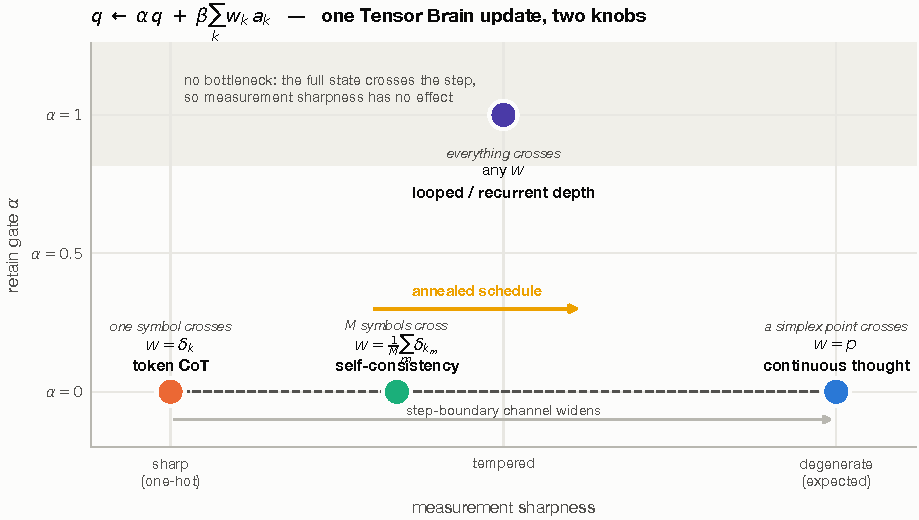
\includegraphics[width=\linewidth]{figures/dial.pdf}
\caption{The two knobs of one Tensor Brain step update. The horizontal axis is
measurement sharpness, which selects the feedback weights $w$ and interpolates
token CoT, self-consistency and continuous thought. The vertical axis is the retain
gate $\alpha$, which decides how much of the latent state survives the step and
therefore whether the index layer is a bottleneck at all. In the shaded band the
sharpness axis has no effect, because nothing is forced through the index layer.}
\label{fig:dial}
\end{figure}

Every intermediate reasoning step in this report applies
\begin{equation}
q \;\leftarrow\; \alpha\,q \;+\; \beta \sum_{k \in \mathcal{K}} w_k\,a_k,
\qquad
p = \operatorname{softmax}(s), \quad s_k = \CBS^{\top}a_k,
\label{eq:dial}
\end{equation}
where $\mathcal{K}$ is the candidate set of the concept window. Conditions differ
only in how $w$ is formed:

\begin{center}
\begin{tabular}{@{}lll@{}}
\toprule
Feedback weights $w$ & Reads as & TB operation \\
\midrule
$w = \delta_{k}$, $k \sim p$        & token CoT, one collapse            & \texttt{measure}, \texttt{sample} \\
$w = \delta_{\arg\max p}$           & greedy CoT                          & \texttt{measure}, \texttt{argmax} \\
$w = \frac1M\sum_{m}\delta_{k_m}$   & $M$ measurements averaged           & --- \\
$w = \operatorname{softmax}(s/\tau)$& tempered / partial collapse         & --- \\
$w = p$                             & continuous thought                  & \texttt{attend} \\
$w = 0$                             & no feedback                         & --- \\
$w \mapsto u$ (fixed vector)        & pause token                         & --- \\
\bottomrule
\end{tabular}
\end{center}

Two of the seven are TB core operations already, and the QTB reading of
\texttt{attend} as a degenerate measurement is what makes the row ordering a
continuum rather than a list. The temperature $\tau$ moves the \emph{bias} of the
estimator (how peaked the distribution being fed back is) and $M$ moves its
\emph{variance} (how well a finite sample represents it); these are separate axes
and we keep them separate throughout.

\begin{remark}[What the unification does and does not assert]
\label{rem:schedule}
That attention and measurement share the form \eqref{eq:dial} is unconditional:
both printed equations have it. Whether the two are \emph{alternatives} is a
separate question on which the two Tensor Brain papers disagree, and we do not
resolve it here. Original TB Section 5.3 introduces the semantic-attention
approximation as replacing the sampled-injection line, making attention an
alternative to measurement. QTB instead states that Algorithm~2 (input and
attention) and Algorithm~3 (generative measurement) execute \emph{sequentially},
so that attention is part of input integration and precedes measurement rather than
standing in for it. This report follows the original's alternative reading, as the
rest of the repository does, and its conditions should therefore be read as a
controlled family of operators rather than as competing Tensor Brain schedules. A
sequential condition, in which attention precedes measurement inside the same
concept window, is the QTB-faithful companion and is not run here.
\end{remark}

\subsection{The step boundary as a channel}
\label{sec:bottleneck}

The knob that the LLM setting hides is $\alpha$. In an autoregressive transformer,
content generated at one step reaches the next only by being written as a token, and
that is a property of the architecture, not a hyperparameter. Equation~\eqref{eq:dial}
exposes it. At $\alpha = 1$ the pre-CBS survives the step intact and the feedback is
an \emph{addition} to an otherwise complete state; at $\alpha = 0$ the state is
\emph{replaced} by the feedback, so everything the chain carries forward has to pass
through $\sum_k w_k a_k$.

This makes the capacity of the step boundary explicit and orderable. A one-hot $w$
transmits one symbol, at most $\log_2|\mathcal{K}|$ bits. An $M$-sample average
transmits a multiset of $M$ symbols. A general $w = p$ transmits a point of the
$(|\mathcal{K}|-1)$-simplex, which is real-valued and can represent a whole frontier
at once. The prediction is immediate and is the main empirical claim of
\S\ref{sec:results-plane}: \emph{measurement sharpness should matter in proportion to
how much the task needs to cross the boundary, and not at all when $\alpha = 1$.}

\subsection{Deferred measurement and the Jensen gap}
\label{sec:jensen}

In unitary quantum computation the deferred-measurement principle says intermediate
measurements can always be postponed to the end of the circuit without changing the
output distribution \citep{nielsen2010quantum}. It holds because the evolution is
linear. The TB evolution operator is not, and this is exactly where discrete and
continuous chains part company.

Write $\bar a = \sum_k p_k a_k$ and $\bar q = \alpha q + \beta \bar a$ for the state
a degenerate measurement produces, and $q_k = \alpha q + \beta a_k$ for the state
outcome $k$ produces. Deferring the measurement means evolving $\bar q$; performing
it means evolving $q_k$ and averaging over $k$.

\begin{proposition}[When measurement may be deferred]
\label{prop:defer}
Let $\Ev$ be continuous on the convex hull $C$ of $\{q_k\}_{k\in\mathcal{K}}$. Then
$\Ev(\bar q) = \Exp_{k\sim p}[\Ev(q_k)]$ for every distribution $p$ on
$\mathcal{K}$ and every $q$ if and only if $\Ev$ is affine on $C$.
\end{proposition}

\begin{proof}
If $\Ev$ is affine the two sides agree by linearity of expectation. Conversely,
taking $p = \tfrac12(\delta_j + \delta_k)$ gives
$\Ev\!\left(\tfrac{x+y}{2}\right) = \tfrac12(\Ev(x) + \Ev(y))$ for all
$x, y \in \{q_k\}$, and applying the same identity to the resulting midpoints
extends it to all dyadic convex combinations, which are dense in $C$. A continuous
solution of Jensen's functional equation on a convex set is affine.
\end{proof}

So the two ends of the dial compute the same thing only in the degenerate case where
the evolution operator does no nonlinear work --- that is, only when the chain is not
reasoning. The size of the discrepancy is second order in the feedback gate.

\begin{proposition}[Second-order gap]
\label{prop:second-order}
If $\Ev$ is twice continuously differentiable at $\bar q$, then
\begin{equation}
\Exp_{k \sim p}\!\left[\Ev(q_k)\right] - \Ev(\bar q)
\;=\;
\tfrac{1}{2}\,\beta^{2}\,
\Big(\tr\!\big(\nabla^{2}\Ev_{j}(\bar q)\,\Cov_p[a]\big)\Big)_{j}
\;+\; O(\beta^{3}),
\label{eq:gap}
\end{equation}
where $\Ev_j$ is the $j$-th output coordinate and
$\Cov_p[a] = \sum_k p_k a_k a_k^{\top} - \bar a\,\bar a^{\top}$.
\end{proposition}

\begin{proof}
Put $\delta_k = a_k - \bar a$, so $q_k = \bar q + \beta \delta_k$ and
$\Exp_p[\delta_k] = 0$. A second-order Taylor expansion of each output coordinate
about $\bar q$ gives
$\Ev_j(q_k) = \Ev_j(\bar q) + \beta\,\nabla \Ev_j(\bar q)^{\top}\delta_k
+ \tfrac{1}{2}\beta^{2}\,\delta_k^{\top}\nabla^{2}\Ev_j(\bar q)\,\delta_k + O(\beta^3)$.
Taking expectations kills the linear term, and
$\Exp_p[\delta_k^{\top} H \delta_k] = \tr(H\,\Cov_p[a])$.
\end{proof}

Two consequences do the work later.

\begin{corollary}[Confidence is free, hedging is not]
\label{cor:confidence}
The leading term of \eqref{eq:gap} vanishes iff $\Cov_p[a] = 0$ on the span of the
candidate embeddings, i.e.\ iff $p$ is a point mass. A chain that is already certain
loses nothing by collapsing; a chain that is hedging loses precisely the
curvature-weighted spread of what it was hedging over.
\end{corollary}

Corollary~\ref{cor:confidence} is the principled version of a heuristic that appears
repeatedly in the latent-reasoning literature --- commit when confident, stay
continuous when uncertain --- and it is what motivates the annealed schedules of
\S\ref{sec:results-schedule}. It also predicts the shape of
Figure~\ref{fig:jensen}(b): the gap should grow with the index entropy of the step,
because entropy and $\tr\Cov_p[a]$ move together for a near-orthonormal index bank.

\subsection{Averaging inside a step is not self-consistency}
\label{sec:mc}

Self-consistency \citep{wang2022selfconsistency} samples whole chains and
marginalises their answers. It is tempting to read continuous thought as the limit of
that procedure. It is not, and Proposition~\ref{prop:second-order} says why.

With $M$ i.i.d.\ draws the feedback is
$\hat f_M = \frac{1}{M}\sum_m a_{k_m}$, an unbiased estimator of $\bar a$ with
covariance $\tfrac1M \Cov_p[a]$, so
\begin{equation}
\Exp\big\|\hat f_M - \bar a\big\| \;=\; \Theta\!\big(M^{-1/2}\big)\sqrt{\tr \Cov_p[a]} .
\label{eq:mc}
\end{equation}
Averaging \emph{inside} a step therefore converges to the continuous update at rate
$M^{-1/2}$: widen the channel enough and a chain of measurements becomes a chain of
continuous thoughts. Averaging \emph{across} chains does something different. Let
$\Ev^{(H)}$ denote $H$ composed steps; self-consistency estimates
$\Exp[\Ev^{(H)}(\cdot)]$ over sampled trajectories, whereas continuous thought
computes $\Ev^{(H)}(\Exp[\cdot])$ step by step. These differ by the Jensen gap
accumulated at every step, and no number of samples closes it. In the language of
\S\ref{sec:jensen}, self-consistency defers nothing and averages at the end;
continuous thought defers everything and never averages.

\subsection{Repeated measurement of one window}
\label{sec:zeno}

The QTB draft raises repeated operator application without fresh input as a model of
deliberation. The dial makes a sharper version available: measure the \emph{same}
concept window several times, with no evolution in between. Writing $R$ for the
number of repeats, the iteration is
\begin{equation}
q_{r+1} = \alpha\,q_r + \beta \sum_k w_k(q_r)\,a_k ,
\label{eq:zeno}
\end{equation}
which is a fixed-point map on a single window. Because feedback re-enters through the
same $A$ that produced the scores, measuring an index raises that index's score, and
the window self-reinforces. This is the mechanism behind the quantum Zeno effect
\citep{misra1977zeno}, where frequent measurement freezes a state, transplanted to a
setting where the ``state'' is a belief over symbolic indices.

Linearising $\sigma(q) - \tfrac12 \approx q/4$ and taking a near-orthonormal index
bank, $A^{\top}A \approx I$, the score iteration becomes
$s \leftarrow \alpha s + \tfrac{\beta}{4}\operatorname{softmax}(s)$.
The maximally uncertain state $s \propto \mathbf{1}$ is a fixed point, and the
Jacobian there is $\alpha I + \tfrac{\beta}{4}(\operatorname{diag}(p) - pp^{\top})$
with eigenvalue $\alpha + \tfrac{\beta}{4K}$ on the subspace orthogonal to
$\mathbf{1}$, where $K = |\mathcal{K}|$.

\begin{proposition}[Commitment threshold, small-signal regime]
\label{prop:zeno}
In this linearisation the uncertain fixed point of \eqref{eq:zeno} is stable iff
$\alpha + \beta/(4K) < 1$; above that threshold repeated measurement drives the
window towards an absorbing one-hot state with no evolution step. For $\alpha < 1$
the non-uniform fixed points satisfy $s^{\star} = \tfrac{\beta}{4(1-\alpha)}\,p(s^{\star})$,
so $\beta/(1-\alpha)$ sets how peaked the window ends up.
\end{proposition}

\begin{remark}[This threshold does not survive contact with the trained model]
\label{rem:zeno-fails}
We state Proposition~\ref{prop:zeno} because it is the natural first analysis and
because it is \emph{wrong} about the regime we actually measure, in an instructive
way. With $K = 64$ it predicts that $\alpha = 0.5$ sits far inside the stable region
for every gate we sweep, so a half-decaying window should not sharpen at all.
Section~\ref{sec:results-zeno} finds that $\alpha = 0.5$ sharpens \emph{fastest}. The
linearisation is at fault: it expands $\sigma$ about the origin, whereas a trained
chain writes states whose norm puts $\sigma$ deep into saturation, and the fixed-point
scale $\beta/(1-\alpha)$ --- which grows as $\alpha$ falls --- dominates the local
stability calculation. The small-signal threshold is therefore not a prediction about
trained Tensor Brains, and we report the repeated-measurement behaviour empirically
instead.
\end{remark}

Whether the resulting commitment is \emph{useful} --- whether the window sharpens
towards the correct answer or merely towards its own first guess --- is not settled by
either calculation, and \S\ref{sec:results-zeno} answers it directly.

\section{Task and setup}
\label{sec:setup}

\paragraph{Task.} We use a TB-native analogue of ProsQA: a fixed layered DAG over
concept nodes, with $400$ start concepts and four subsequent layers of $64$ nodes
each, branching factor $2$. A query writes a start concept and two candidate terminal
concepts into the workspace; exactly one terminal is reachable, and the model must
say which. The graph is fixed across the whole dataset, so it is knowledge that has to
live in the model rather than in the input.

\paragraph{Removing the shortcuts.} Two controls make the task about traversal rather
than association, and both were necessary --- earlier versions of this study produced
uniformly high accuracy for every condition until they were added.
\begin{itemize}
\item \emph{Quota-balanced negatives.} A terminal that many starts reach is, for that
reason, rarely available as somebody else's unreachable option, so matching negatives
on in-reachability count is not enough. Negatives are assigned under a quota making
each terminal occupy the correct and incorrect slot equally often. A terminal-identity
rule fitted on the training split then scores \TerminalShortcut on the held-out
split, i.e.\ noise.
\item \emph{Frozen index bank.} A trainable $A$ of realistic size simply stores
(start, terminal) associations and answers without traversing, at which point every
collapse condition scores identically. We therefore freeze $A$ to a fixed random code.
All task knowledge lives in the evolution operator, and superposition readout is the
only route to the answer.
\end{itemize}
Splits are over distinct reachable (start, terminal) pairs, so every start and every
terminal is seen in training but their composition is not.

\paragraph{Supervision and curriculum.} Intermediate steps here are inherently
multi-valued: several children of the current frontier are equally valid
continuations, so a one-hot ``gold path'' target is misspecified and teaches an
arbitrary tie-break. We supervise instead towards the true breadth-first
\emph{frontier} at each hop. Training follows COCONUT's staged curriculum: at stage
$k$ the first $k$ intermediate hops use the condition's own collapse and the rest are
teacher-forced onto the true frontier, with step loss only at teacher-forced hops.
The teacher is a \emph{distribution}, not a node: writing back a single gold node
would put one path in the workspace while the step target is the whole frontier, a
target that state cannot support, and getting this wrong was what kept an earlier
version of the chain from learning at all. Teacher forcing is training-only and never
an evaluation condition, since writing the true frontier into the workspace leaks the
answer. Reaching any nontrivial accuracy required this curriculum, independently
matching the necessity argument of \citet{zou2026limits}.

\paragraph{Model and controls.} A single shared evolution operator (QTB
Algorithm~1, one sigmoid hidden layer of $1024$ units on a $384$-dimensional
pre-CBS) is applied at every hop; the candidate set at hop $h$ is layer $h$,
identically across conditions. Discrete modes use a straight-through estimator
\citep{bengio2013estimating,jang2017gumbel} with the tempered softmax as surrogate.
Two controls separate ``more compute'' from ``more information'': \emph{no feedback}
($w=0$) and a \emph{pause vector} (a learned direction independent of the candidate
distribution), the analogue of pause tokens \citep{goyal2023pause}.

\paragraph{A confound worth naming.} A flat $w$ averages many near-orthogonal
embeddings towards zero, so soft feedback is intrinsically smaller in norm than a
one-hot collapse --- in our setting by roughly $9\times$. Comparing them naively
confounds measurement sharpness with how hard the step pushes on the state. We
rescale all feedback to a common norm before applying $\beta$, so that the dial
varies direction and not magnitude.

\section{Results}

\subsection{Sharpness matters only at the bottleneck}
\label{sec:results-plane}

\begin{figure}[t]
\centering
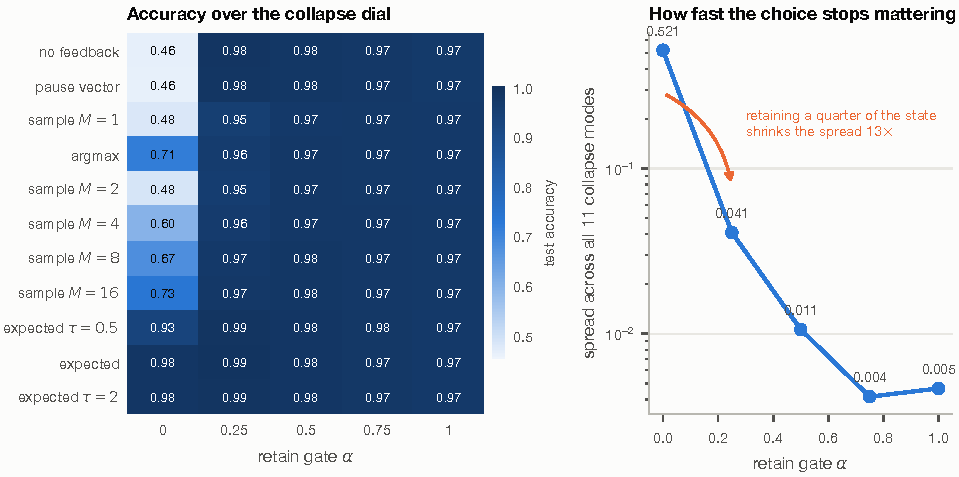
\includegraphics[width=\linewidth]{figures/plane.pdf}
\caption{Test accuracy over the collapse dial, \NumSeeds\ seeds, \NumTestQueries\
held-out queries. \textbf{Left:} the full grid of retain gate against collapse mode.
Only the $\alpha = 0$ column varies; everywhere else the choice of collapse is worth
less than a percentage point. \textbf{Right:} the spread across all eleven modes as a
function of $\alpha$, on a log axis. The dependence is steep rather than gradual ---
retaining a quarter of the state already removes most of the effect.}
\label{fig:plane}
\end{figure}

Figure~\ref{fig:plane} is the central result. At $\alpha = 1$ every condition lands
in a band \OpenMeanSpread wide --- including \emph{no feedback}, which never touches
the index layer at all. Whatever the chain needs is already carried by the pre-CBS,
so the measurement is decorative and its sharpness is not a variable.

At $\alpha = 0$ the same eleven conditions spread over \BottleneckMeanSpread, and
they order themselves by how much the collapse can transmit and by nothing else. The
no-feedback and pause controls sit at chance (\BottleneckNoFeedback and
\BottleneckPause); a single sampled symbol is barely above it
(\BottleneckSampleOne); the $M$-sample average climbs monotonically with $M$
(\BottleneckSampleOne, $0.482$, $0.595$, $0.674$, \BottleneckSampleSixteen for
$M = 1, 2, 4, 8, 16$); and the exact expectation reaches \BottleneckContinuous. The
temperature axis moves the same way in isolation: $\tau = 2$ and $\tau = 1$ are
indistinguishable at $0.979$ and \BottleneckContinuous, $\tau = 0.5$ falls to $0.926$,
and the hard limit reaches \BottleneckArgmax. That the pause control fails while the
same number of evolution steps with informative feedback succeeds is what rules out
``extra compute'' as the explanation, exactly as pause tokens do in the LLM setting.

Two details are worth more than the ordering itself.

\paragraph{The transition is abrupt, not gradual.} We expected the spread to close
smoothly as $\alpha$ rose. It does not. Retaining a mere quarter of the pre-CBS
shrinks the spread across all eleven modes from \BottleneckMeanSpread to
\QuarterMeanSpread, a factor of thirteen, and by $\alpha = 0.75$ it is under
$0.005$ --- a factor of $130$. Whatever the step boundary is doing, it is close to an
on/off switch rather than a dial in this dimension, even though the sharpness axis
\emph{is} a smooth dial at $\alpha = 0$. The practical form of this claim is
falsifiable outside the Tensor Brain: any architecture that carries even a fraction
of its reasoning state across the step boundary --- a residual path, a persistent
cache, a recurrent hidden state --- should be correspondingly insensitive to whether
its intermediate steps are decoded discretely, and the discrete-versus-continuous
question should only bite where the boundary is close to total.

\paragraph{Feedback can be worse than none.} At $\alpha = 0.25$ the best condition is
\emph{no feedback} at $0.983$, ahead of a single sampled measurement at $0.947$. Once
the retained state already carries the frontier, writing a sampled index back into it
adds noise to a sufficient statistic. Measurement is not free even when it is cheap,
which is a second reason not to read the collapse dial as ``more symbolic grounding is
better''.

\subsection{Is it the gate, or the capacity?}
\label{sec:results-capacity}

\begin{figure}[t]
\centering
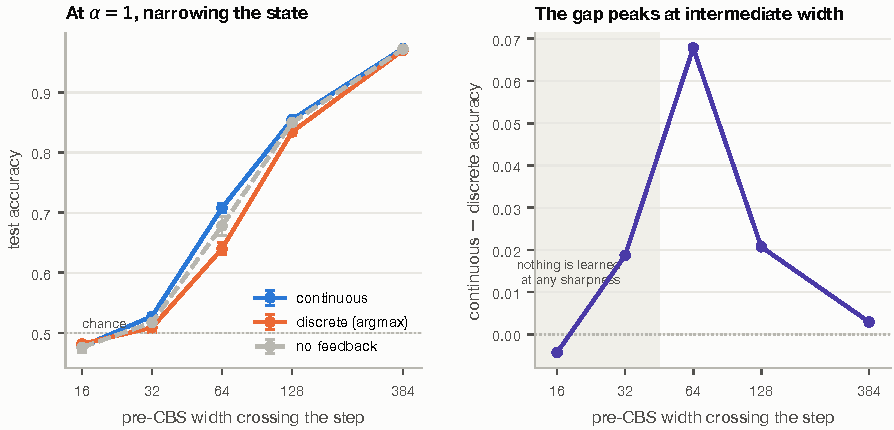
\includegraphics[width=\linewidth]{figures/capacity.pdf}
\caption{Holding $\alpha = 1$ and narrowing the pre-CBS that crosses the step.
\textbf{Left:} the three headline conditions against state width.
\textbf{Right:} the continuous minus discrete accuracy gap. If the $\alpha = 1$ null
were about the retain gate as such it should persist at every width; if it is about
how much information the boundary can carry, the conditions should separate again
once the state is too narrow to hold the frontier.}
\label{fig:capacity}
\end{figure}

Section~\ref{sec:results-plane} is easy to over-read. What crosses the boundary at
$\alpha = 1$ is a $384$-dimensional state, comfortably wider than the frontier this
task needs; what crosses at $\alpha = 0$ under a one-hot collapse is about
$\log_2 64 = 6$ bits. Both knobs may therefore be moving one underlying quantity,
the capacity of the step boundary, with $\alpha$ merely the coarser of the two.
Figure~\ref{fig:capacity} tests this directly by holding $\alpha = 1$ and shrinking
the pre-CBS.

The answer is a qualified yes, and the qualification is the interesting part. The gap
between continuous and discrete feedback traces an inverted U in state width. It is
$0.003$ at $384$ dimensions, rises to \CapacityPeakGap at \CapacityPeakDim
dimensions --- roughly twenty times larger --- and falls back to nothing at $16$--$32$
dimensions, where no condition exceeds \CapacityFloorAccuracy and the model simply
fails to learn the task at all. Read past that floor, the middle of the curve is a
genuine confirmation: the $\alpha = 1$ null is not a property of the retain gate, and
narrowing what survives the step brings the collapse modes apart again.

What the sweep also shows is that the two axes are \emph{not} interchangeable. The
largest gap narrowing alone can produce is \CapacityPeakGap, while replacing the state
with a single symbol at $\alpha = 0$ produces $0.277$. A $64$-dimensional continuous
state and a $6$-bit symbol are both small, but the first still holds graded evidence
about many candidates at once and the second holds one node. Capacity in bits is the
wrong summary; what the boundary must be able to carry is a \emph{superposition}, and
dimension buys that where discreteness forecloses it. We would therefore resist
collapsing the two knobs of Figure~\ref{fig:dial} into a single scalar, and read
Figure~\ref{fig:capacity} as showing that they are correlated rather than the same.

\subsection{Widening the channel}
\label{sec:results-mc}

\begin{figure}[t]
\centering
\begin{subfigure}{0.48\linewidth}
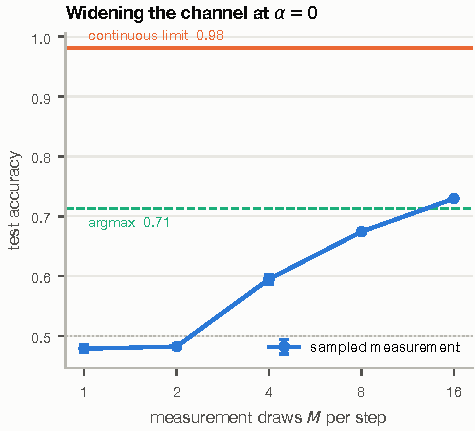
\includegraphics[width=\linewidth]{figures/channel.pdf}
\caption{Accuracy against draws per step.}
\end{subfigure}\hfill
\begin{subfigure}{0.48\linewidth}
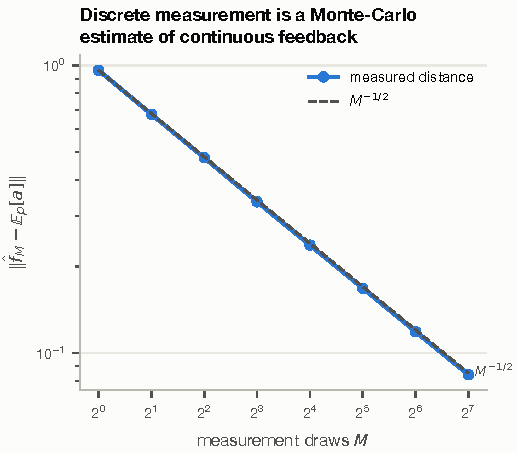
\includegraphics[width=\linewidth]{figures/mean_field.pdf}
\caption{Feedback distance to the exact expectation.}
\end{subfigure}
\caption{Averaging measurements inside a step. (b) confirms the $M^{-1/2}$ rate of
\eqref{eq:mc} with the expectation computed exactly over the candidate set.}
\label{fig:channel}
\end{figure}

Figure~\ref{fig:channel} tracks the estimator directly, and \eqref{eq:mc} is met
almost exactly. Going from $M = \MCFirstSamples$ to $M = \MCLastSamples$ draws, the
distance between the sampled feedback and the exact expected feedback falls from
\MCFirstDistance\ to \MCLastDistance, a ratio of \MCObservedRatio\ against the
$\sqrt{\MCLastSamples} = \MCPredictedRatio$ the rate predicts. Accuracy rises with
$M$ in step, from \BottleneckSampleOne\ at a single draw to \BottleneckSampleSixteen\
at sixteen, against \BottleneckContinuous\ for the exact expectation.

This is the sense in which continuous thought is the mean-field limit of repeated
measurement. It is worth being precise about what it is \emph{not}. Self-consistency
\citep{wang2022selfconsistency} also averages many sampled chains, and it is tempting
to read latent reasoning as its limit; \S\ref{sec:mc} says otherwise. Averaging inside
a step converges here at $M^{-1/2}$ because the object being averaged is the feedback
vector, which enters the next evolution linearly. Averaging across whole trajectories
composes the nonlinear $\Ev$ before averaging, and by Proposition~\ref{prop:defer}
that limit differs from the continuous chain by the Jensen gap accumulated at every
step --- no number of samples closes it. The two procedures look alike and converge to
different things.

\subsection{Measurement does not commute with evolution}
\label{sec:results-jensen}

\begin{figure}[t]
\centering
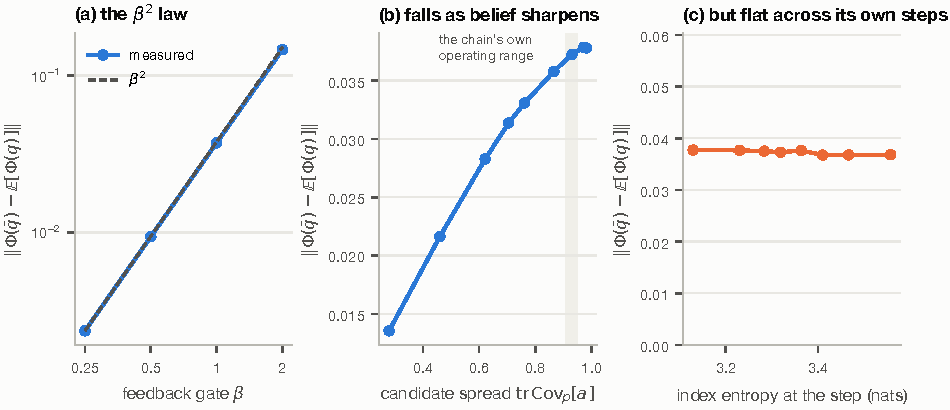
\includegraphics[width=\linewidth]{figures/jensen.pdf}
\caption{The Jensen gap between evolving the averaged state and averaging the evolved
states, computed exactly over the candidate set. \textbf{(a)} the predicted
$\beta^{2}$ law of Proposition~\ref{prop:second-order}. \textbf{(b)} tempering the
chain's own scores sweeps the candidate spread across its full range; the gap falls
steeply towards zero as $p$ sharpens, in the direction Corollary~\ref{cor:confidence}
requires, and the shaded band marks where the trained chain's own steps actually sit.
\textbf{(c)} bucketing those steps by entropy instead gives a flat line --- not a
refutation, but a range problem, since the spread is saturated everywhere in (b)'s
shaded band.}
\label{fig:jensen}
\end{figure}

One scope note. Propositions~\ref{prop:defer} and \ref{prop:second-order} are
statements about the printed update $q \leftarrow \alpha q + \beta\sum_k w_k a_k$, and
that is the operator measured here, evaluated at states a trained chain actually
visits. The chain \emph{conditions} instead apply the norm-matched variant of
\S\ref{sec:setup}, so that the dial varies direction rather than magnitude. The two
coincide up to the per-step rescaling, and the $\beta$ sweep below should be read as
characterising the operator, not as a sweep of the trained model's own gate.

The $\beta^{2}$ law of Proposition~\ref{prop:second-order} holds almost exactly:
across the swept gates the measured gap ratios deviate from the predicted factor of
four by at most \JensenQuadraticError\%. This is the quantitative content of the
claim that latent and token reasoning are not two implementations of the same
computation --- the difference is a number, and it is computable at every step.

Corollary~\ref{cor:confidence} fares less simply, and the way it fails is
informative. Bucketing the trained chain's own steps by index entropy gives an
essentially \emph{flat} gap (Figure~\ref{fig:jensen}c): entropy \JensenLowEntropy to
\JensenHighEntropy nats moves it by a ratio of \JensenGapRatio. That is not a
refutation of the corollary, which predicts the gap vanishes when
$\Cov_p[a] \to 0$, i.e.\ at a \emph{point mass} --- and on a search task the chain is
never anywhere near one. Its candidate spread sits at $0.91$--$0.95$ of the maximum
at every step, so entropy varies while the quantity the theory actually names does
not, and the cross-section has no range to test over. Driving the spread across its
full range by tempering the chain's own scores (Figure~\ref{fig:jensen}b) recovers
the predicted behaviour: the gap collapses towards zero as $p$ sharpens.

The practical reading is worth stating plainly, because it explains a result three
sections below. On this task collapse is \emph{never} cheap: the chain never becomes
confident enough for the second-order term to shrink, so there is no step at which
committing is close to free. That is exactly why no annealed schedule in
\S\ref{sec:results-schedule} beats staying continuous throughout, and it predicts
that ``commit when confident'' will only pay on tasks whose intermediate steps
actually become confident --- arithmetic, plausibly, rather than search.

\subsection{Reading the superposition off the index layer}
\label{sec:results-frontier}

\begin{figure}[t]
\centering
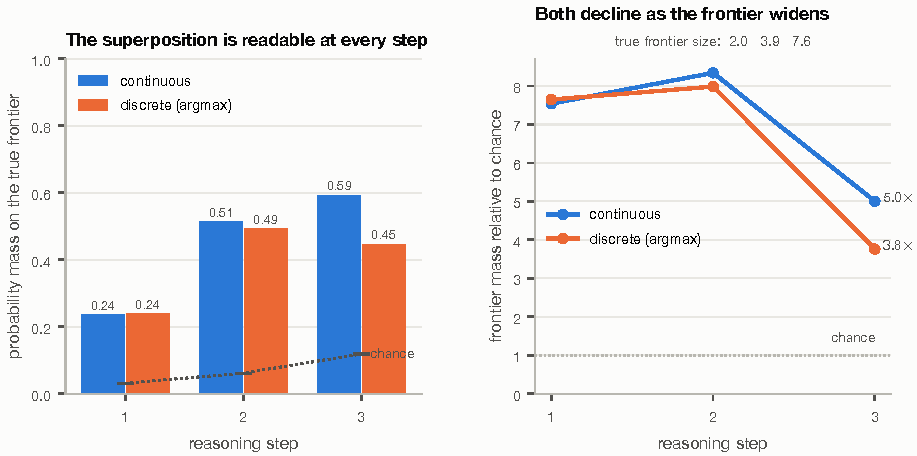
\includegraphics[width=\linewidth]{figures/frontier.pdf}
\caption{\textbf{Left:} probability mass on the true breadth-first frontier at each
step, for a continuous and a discrete chain. \textbf{Right:} effective number of
alternatives $e^{H}$ kept open, against the true frontier size.}
\label{fig:frontier}
\end{figure}

The TB gives this analysis for free. In an LLM the continuous thought has to be
decoded with a Logit Lens or a trained probe to see what it contains; in the TB the
index layer is present at every step by construction, so the candidate distribution
\emph{is} the readout, with no probe to validate and nothing to trust on faith.

What it shows is more specific than ``continuous chains represent more''. Both chains
put far more mass on the true frontier than chance (\FrontierChance), and at the first
two steps they are close to indistinguishable --- $0.236$ against $0.239$ at step one,
$0.514$ against $0.492$ at step two. They separate only at step three, where the
frontier is widest, at $0.593$ against $0.446$. Yet the accuracy difference between
these two chains is enormous: \FrontierMassContinuous\ against
\FrontierMassDiscrete\ mean frontier mass corresponds to $0.983$ against $0.706$ test
accuracy.

That mismatch is the point, and it sharpens the interpretation of
\S\ref{sec:results-plane}. The discrete chain is not much worse at \emph{knowing}
where the search could be; its index distribution is nearly as informative. It is
worse at \emph{transmitting} that knowledge across the step boundary, because a
one-hot collapse can forward only one node of a frontier that by step three averages
$7.6$. The deficit created by measuring sharply is a communication deficit, not a
representational one --- which is exactly why widening the channel in
\S\ref{sec:results-mc} recovers the accuracy without changing anything about what the
chain believes.

\subsection{Search depth}
\label{sec:results-depth}

\begin{figure}[t]
\centering
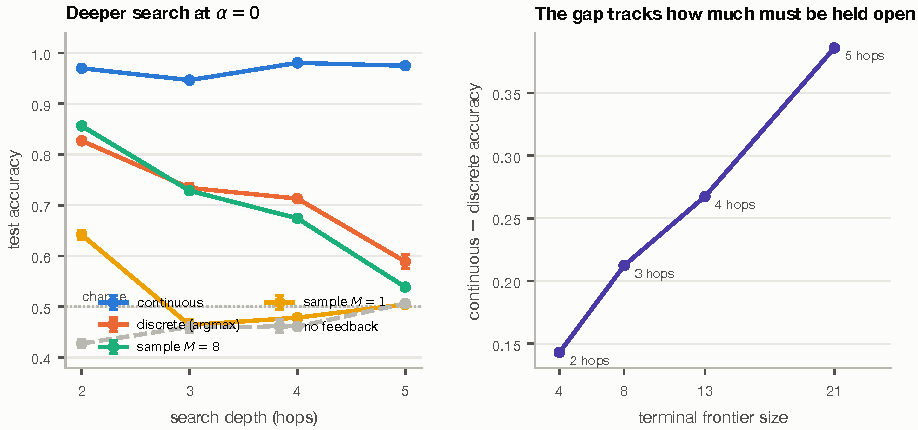
\includegraphics[width=\linewidth]{figures/depth.pdf}
\caption{Search depth at $\alpha = 0$, three seeds. \textbf{Left:} continuous feedback
is flat in depth while every discrete condition decays. \textbf{Right:} the gap
against the size of the terminal frontier the chain has to represent.}
\label{fig:depth}
\end{figure}

If the deficit created by sharp measurement is a communication deficit, it should
scale with how much there is to communicate. Figure~\ref{fig:depth} varies the search
depth from \DepthShallow\ to \DepthDeep\ hops, which grows the terminal frontier from
\DepthFrontierShallow\ nodes to \DepthFrontierDeep.

The continuous chain is essentially \emph{depth-invariant}: it scores between
\DepthContinuousMin\ and \DepthContinuousMax\ at every depth, because carrying a
frontier of twenty-one costs it no more than carrying a frontier of four. Every
discrete condition decays monotonically, and the gap grows from \DepthGapShallow\ to
\DepthGapDeep\ --- close to linear in frontier size over this range.

The $M$-sample condition dates the mechanism precisely. An $M$-draw collapse forwards
at most $M$ distinct nodes, so it should track the continuous chain while
$M$ exceeds the frontier and fall away once it does not. At $M = 8$ that crossing
should happen between three and four hops, and it does: \DepthSampleEightShallow\ at
a frontier of four, then \DepthSampleEightDeep\ at a frontier of twenty-one. This is
the same $M$ axis as \S\ref{sec:results-mc}, now with the frontier rather than the
sample count as the moving part, and it agrees.

\subsection{Where in the chain to collapse}
\label{sec:results-schedule}

\begin{figure}[t]
\centering
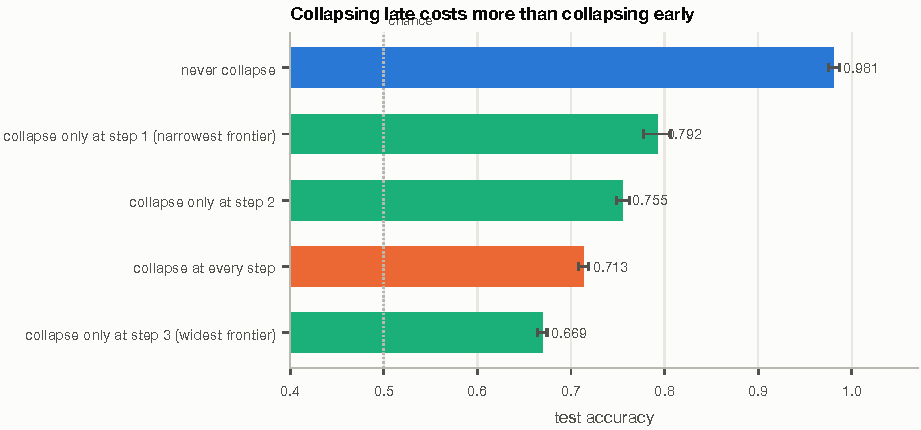
\includegraphics[width=0.62\linewidth]{figures/schedule.pdf}
\caption{Where a chain collapses, at $\alpha = 0$. The three middle bars each
collapse exactly once, at the first, second and third reasoning step respectively;
the frontier widens with depth, so the same single collapse costs more the later it
lands. Collapsing at every step beats collapsing only at the last.}
\label{fig:schedule}
\end{figure}

Corollary~\ref{cor:confidence} says collapse is free when the step is confident and
expensive when it is not. The frontier widens with depth on this task, so the
prediction is that \emph{where} a chain collapses should matter as much as whether it
does, and that collapsing early should cost less than collapsing late.

Figure~\ref{fig:schedule} bears this out sharply. Among the three schedules that
collapse exactly once, accuracy is monotone in the position of that collapse:
\SchedEarly at the first step, \SchedAlternating at the second, \SchedLate at the
third, against \SchedNeverCollapse for a chain that never collapses. One collapse
step is not one cost; it is a cost that scales with how much was being held open when
it landed.

The comparison we did not anticipate is more interesting. Collapsing at
\emph{every} step (\SchedAlways) is \emph{better} than collapsing only at the last
one (\SchedLate). A chain that measures throughout is trained to work from single
nodes and never builds a superposition it cannot transmit; a chain that stays
continuous and then collapses immediately before readout spends three steps
assembling a frontier and discards it at the one moment it was needed. Consistency
between what the chain represents and what the step boundary can carry is worth more
than continuity at any individual step, which is a caution against bolting a discrete
decoding step onto the end of an otherwise latent reasoner.

\subsection{Repeated measurement of one window}
\label{sec:results-zeno}

\begin{figure}[t]
\centering
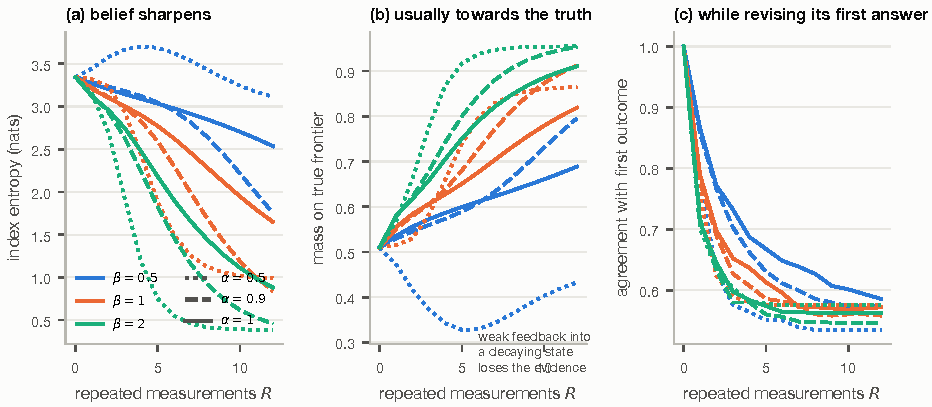
\includegraphics[width=\linewidth]{figures/zeno.pdf}
\caption{Repeated measurement of a single concept window, with no evolution and no
new input in between, across nine $(\alpha,\beta)$ settings. \textbf{(a)} the index
distribution sharpens in every setting, including ones
Proposition~\ref{prop:zeno} calls stable. \textbf{(b)} in eight of nine settings the
sharpening moves \emph{towards} the true frontier; the exception is weak feedback
into a decaying state, where the evidence washes out faster than it accumulates.
\textbf{(c)} agreement with the window's own first outcome falls to about $0.57$ and
stays there, so this is revision rather than self-reinforcement.}
\label{fig:zeno}
\end{figure}

This is the operation the QTB draft gestures at, and on this task it works. Holding
one concept window fixed and measuring it \ZenoRepeats times with no evolution and no
new perceptual input, the index entropy falls from \ZenoEntropyStart to
\ZenoEntropyEnd nats, and --- the part that matters --- probability mass on the true
frontier rises from \ZenoFrontierStart to \ZenoFrontierEnd. The window does not merely
become more certain; it becomes more \emph{right}, at the cost of no evolution steps
whatsoever.

Two controls establish that this is deliberation rather than a self-fulfilling loop.
First, agreement with the window's own first outcome falls to roughly $0.57$ and
plateaus (Figure~\ref{fig:zeno}c): in over forty percent of queries the window ends up
committed to a different index than the one it would have named initially, so the
feedback is not simply amplifying whatever it happened to see first. Second, the
improvement is not automatic. At $\alpha = \beta = 0.5$ --- weak feedback written into
a state that halves every repeat --- frontier mass \emph{falls} from $0.51$ to $0.33$
before partially recovering. Repeated measurement helps only when what it writes back
accumulates faster than the retained state decays.

We flag the obvious caveat: these trajectories are read from a chain trained with a
single measurement per window, so they show what repeated measurement does to a
representation that was not optimised for it. Training under a repeated-measurement
schedule is the natural follow-up and is not run here.

\section{Discussion}

\paragraph{The question is about the channel, not the representation.} The result we
would most like to carry over is the $\alpha$ finding. Discussions of latent reasoning
usually compare a discrete pipeline against a continuous one and attribute the
difference to the representation. Equation~\eqref{eq:dial} says the representation
matters only in proportion to how much of the state is destroyed at the step boundary,
and that the dependence is steep: a quarter of the state retained is already most of
the way to not mattering. For transformers this suggests the useful question is not
``discrete or continuous?'' but ``how much of the reasoning state actually has to
survive re-entry?'', and architectures differ in that far more than in the sharpness
of their decoding. It also suggests a cheap diagnostic. Before asking whether a system
would benefit from latent reasoning, measure how much of its reasoning state already
crosses its step boundary; if the answer is ``most of it'', the continuous variant has
little room to help, whatever the benchmark says.

\paragraph{Two knobs, not one.} We were tempted to collapse $\alpha$ and sharpness
into a single scalar capacity, and \S\ref{sec:results-capacity} says not to. Narrowing
a continuous state and discretising it are both ways of shrinking what crosses the
boundary, but they are not equivalent at equal nominal size, because only one of them
can still carry a superposition. Whatever the right currency for step-boundary
capacity is, it is not bits.

\paragraph{Deferred measurement as a design principle.} Proposition~\ref{prop:defer}
gives a clean way to think about when a reasoning system may postpone its decisions.
It may, exactly to the extent that its dynamics are affine over the alternatives it is
entertaining. Everything a nonlinear reasoner gains by staying continuous, and
everything it risks, is in the second-order term.

\paragraph{Limitations.} These are from-scratch models on one synthetic task with a
frozen random index bank, chosen precisely so that the phenomenon under study is not
confounded by memorisation; \citet{rizvimartel2026illusion} give good reason to expect
fine-tuned LLMs to behave differently, and nothing here transfers automatically to
them. The task is reachability, where superposition has a known and provable advantage
\citep{zhu2025superposition}; the arithmetic side of COCONUT's split, where continuous
reasoning \emph{loses}, is not modelled here at all and is the obvious next test of
whether the $\alpha$ account generalises. The Zeno analysis is a linearisation plus a
numerical sweep, not a proof about the trained operator. Finally, $\tau$ and $M$ were
swept at evaluation and training together; disentangling train-time and test-time
sharpness, as \citet{butt2025softtokens} do, is left open.

\paragraph{What would need a cluster.} Everything above runs on a laptop CPU. Three
extensions would not: a branching-factor sweep wide enough to estimate the exponent
relating frontier size to the discrete--continuous gap; an arithmetic-style task with
a genuine computational rather than search bottleneck, to test whether the ordering
inverts as it does between ProsQA and GSM8k; and porting the $\alpha$ sweep to a small
transformer, where the retain gate would have to be introduced deliberately because
the architecture does not provide it.

\bibliography{refs}

\end{document}
